\chapter{The Research Project}\label{C:aim}

In this chapter, we outline the main ideas and objectives of this research project. 
%%% ACF Only complexity?
Section~\ref{Sec:AdvantagesLimitations} discusses entropy and complexity analysis in time series, highlighting its advantages and limitations. 
%%% ACF Use numbered sections/subsections and refer to their automatic numbers
Section~\ref{Sec:BP method} examines the advantages and  limitations of the Bandt and Pompe method. 
Section~\ref{Sec:BackgroundKnowledge}  provides background knowledge on the 
%%% ACF What is this plane?
entropy-complexity plane. 
Section~\ref{Sec:EntropyComplexity} explores the entropy-complexity plane for a broad class of time series. Section~\ref{Sec:AsymptoticDistribution} provides the asymptotic distribution of the entropy. Finally, the chapter concludes with the objectives of the research project and a case study related to our work.

%%% ACF Do you analyse complexity only?
\section{Entropy and Complexity Analysis in Time Series: Advantages and Limitations}\label{Sec:AdvantagesLimitations}

Entropy and complexity analysis in time series provides powerful tools for measuring the unpredictability and structural richness of dynamical systems, which means the systems that evolve in time. 
These methods help describe the behavior of a system using mathematical models. 
%%% ACF What's the difference between SE and PE?
Entropy measures, such as Shannon entropy (which quantifies the uncertainty in a probability distribution) and permutation entropy (which measures the complexity of the order structure in time series using ordinal patterns), are used to quantify the degree of randomness or disorder in data. 
The major difference between Shannon entropy and permutation entropy is that permutation entropy is the Shannon entropy computed from the ordinal patterns (permutations) extracted from a time series.
The complexity measures assess the balance between order and chaos.  
%%% ACF What is a nonlinear pattern?
Entropy and complexity measures are powerful tools for identifying nonlinear patterns in time series data, and together, they are particularly valuable for distinguishing between deterministic and stochastic behavior by revealing hidden structures and irregular dynamics that traditional linear methods often overlook.
%However, their effectiveness depends heavily on parameter choices, such as embedding dimension and time delay. 
%%% ACF Several problems with the following sentence. (1) at some point, we will say that OPs are little sensitve to outliers, (2) we don't know what "data length" means
%They can be sensitive to noise and data length. 
%%% ACF Rethink the following assertion. I tend to disagree. Computing these quantities is not computationally intensive; but computing their statistical properties taking into account the serial correlation is
%%% ACF What is a high dimensional system?
%%% ACF What is a multi-scale system?
While entropy and complexity analysis offers powerful insights into non-linearity and chaos, capturing patterns that traditional linear methods often miss, it requires careful preprocessing, precise parameter tuning, and a solid understanding of the system's domain to avoid misleading conclusions. Non-linearity refers to relationships within the data where small changes in input can lead to disproportionately large or unpredictable changes in output, often seen in complex real-world systems such as biological signals or financial markets. Choosing the right parameters, such as embedding dimension and time delay, is crucial for accurately capturing the underlying dynamics, and without domain knowledge, interpreting the results and identifying meaningful patterns can be challenging.
% ACF What is a "linear method"?
Despite these limitations, entropy and complexity remain essential in modern time series analysis for uncovering hidden dynamics beyond the reach of traditional linear methods. Linear methods, such as auto-correlation, linear regression, and Fourier analysis, assume that relationships within data are proportional and predictable, often focusing on averaged behavior, periodicity, or stationary patterns. However, many real-world systems (like the brain, heart, or climate) display nonlinear behavior, where the output does not change in a simple, direct way with the input. Entropy and complexity measures are specifically designed to capture these irregularities, revealing subtle structures, transient changes, or chaotic patterns that linear tools often overlook or misinterpret. This makes them invaluable for exploring complex, dynamic, and nonlinear systems where traditional approaches fall short.

%While this method effectively captures ordinal relationships between data points, it has notable drawbacks. 
%First, it ignores amplitude information in the time series. 
%%% ACF "complexity-entropy plane"?
%Second, classifying data via the entropy-complexity plane becomes challenging (or even misleading) in high-dimensional chaotic systems, 
%%% ACF Do you know what chaotic systems are?
%chaotic system is a deterministic dynamical system which shows complex system. There is no random behaviours and the long term process is not repeating the same patterns. 
%%% ACF Read and study about the logistic map.
% Deterministic means that the process always depend on the initial condition and it cannot see the repeated solutions.
%%% ACF What is surrogate data? Surrogate data refers to artificial time series generated from an original data set, which preserve certain properties of the original (like mean, variance, or power spectrum), but are otherwise randomized or restructured. We use surrogate data to test whether patterns in data are truly nonlinear/chaotic, or just due to random chance or noise.
%as both deterministic chaotic time series and stochastic surrogate data may occupy overlapping regions within the plane.

%%% ACF I think that when you refer to "statistical complexity measures" you are referring to "information theory-based measures"
%Despite these limitations, entropy-complexity plane offers a robust framework to enhance ordinal pattern analysis. 
%%% ACF Not only from the (marginal) distribution, but also from the independence
%%% ACF What a dynamical proces is?
%These measures quantify deviations from uniform ordinal pattern distributions, enabling a more nuanced characterization of dynamical processes. 
%%% ACF Cite your sources, otherwise the text is yours
%By combining permutation entropy with statistical complexity, researchers gain a refined tool to differentiate stochastic signals from deterministic chaos, thereby revealing intricate structural patterns and degrees of randomness in time series data.

\section{The Bandt and Pompe Method: A Robust Approach} \label{Sec:BP method}

%%% ACF Reserve "demonstrate" for mathetical proofs
The concept of ordinal patterns in time series can be effectively studied through real world examples. 
Traditionally, numerous algorithms, techniques, and heuristics have been employed to estimate complexity measures from real world data. 
%%% ACF What is a low-dimensional dynamical system? the number of state variables or dimensions are small, we called it as low dimension. 1D, 2D or 3D can be considered as low dimension. 

However, these methods often perform well only for low-dimensional dynamical systems and struggle when noise is introduced. Low-dimensional dynamical systems are systems whose behavior can be described using a small number of variables or equations, typically two or three, such as the logistic map, or pendulum. These systems exhibit rich and often chaotic dynamics but remain mathematically tractable and easier to analyze using entropy and complexity measures. Because of their limited dimensionality, the patterns within the data are more distinct, making it easier to extract meaningful information. 

%%% ACF What is the Lyapunov exponent? It is one of the complexity parameters. It measures how small changes grow over time. 
The Bandt and Pompe method overcomes this limitation by providing a robust approach that remains reliable even in noisy environments. 
In time series analysis, key complexity parameters such as entropy, fractal dimension, 
%%% ACF If you mention it, you must  be able to define it
and Lyapunov exponents play a crucial role in comparing neighboring values and uncovering the underlying structure and dynamics of the data. A Lyapunov exponent measures the average rate at which nearby trajectories in a dynamical system diverge or converge. It provides deeper understanding of system's behavior. 

The advantages of Bandt \& Pompe methods:
\begin{itemize}
	\item Simplicity
	\item Extremely fast calculation
	\item Robustness
	\item Invariance to nonlinear monotonous transformations
\end{itemize}	

This method exhibits low sensitivity to noise and naturally accounts for the causal order of elements in a time series. As a result, it can be applied to various real-world problems, particularly in differentiating between chaotic and stochastic signals.

Despite its limitations, researchers have developed extensions to the original method to address its shortcomings and enhance its applicability to a broader range of complex systems.

\section{Statistical Complexity measures} \label{Sec:BackgroundKnowledge}

Bandt and Pompe introduced a highly effective method for analyzing time series within this framework. They calculated Shannon entropy based on the histogram of causal patterns and successfully identified chaotic components in sequences of words, among other applications.

Later, Rosso et al.~\cite{EEGAnalysisUsingWaveletBasedInformationTools} expanded this analysis by introducing an additional dimension: the statistical complexity derived from the same histogram of causal patterns. The authors have contributed to a wide range of applications. This approach, which utilizes the entropy-complexity plane, has been successfully applied to the visualization and characterization of different dynamical regimes as system parameters change  \cite{Bandt2005,Cao2004,DeMicco2012a,Kowalski2007,Kowalski2011b,Rosso2010a,Zunino2010a,Zunino2012a}, as well as to optical chaos \cite{Liu2016f,Soriano2011a,Toomey2014,Yang2015e,Zunino2011a}, hydrology \cite{Lange2013,Serinaldi2014,Stosic2016}, geophysics \cite{Consolini2014,Saco2010,Sippel2016}, engineering \cite{Aquino2017,Aquino2015,Redelico2017a,Yan2012}, biometrics \cite{Rosso2016}, characterization of pseudo-random number generators \cite{DeMicco2008,DeMicco2009}, biomedical signal analysis \cite{Li2014b,Li2008b,Li2007,Liang2015b,Montani2015a,Montani2014,Montani2014a,Montani2015,Morabito2012,Parlitz2012,Perinelli2025,Perinelli2019,Zanin2012}, and econophysics \cite{Bariviera2015a,Bariviera2015,Bariviera2016,Zanin2012,Zunino2016a,Zunino2009,Zunino2010}, to name a few.

%%% ACF What is system parameter change? It means altering one of the constants in the dynamical system and this can cause the system's behavior to shift drastically.
%system parameter change
%%% ACF Sort the citation number
%%% ACF You must have an idea of every paper you cite
%\cite{Bandt2005,Cao2004,DeMicco2012a,Kowalski2007,Kowalski2011b,Rosso2010a,Zunino2010a,Zunino2012a}, 
%%% ACF What is optical chaos: It refers to chaotic behavior, i.e., unpredictable and highly sensitive to initial conditions, optical system which involves light, such as lasers, or optical fibers.
%optical chaos \cite{Liu2016f,Soriano2011a,Toomey2014,Yang2015e,Zunino2011a}, hydrology \cite{Lange2013,Serinaldi2014,Stosic2016}, geophysics \cite{Consolini2014,Saco2010,Sippel2016}, engineering \cite{Aquino2017,Aquino2015,Redelico2017a,Yan2012}, biometrics \cite{Rosso2016}, characterization of pseudo-random number generators \cite{DeMicco2008,DeMicco2009}, biomedical signal analysis \cite{Li2014b,Li2008b,Li2007,Liang2015b,Montani2015a,Montani2014,Montani2014a,Montani2015,Morabito2012,Parlitz2012,Zanin2012}, econophysics \cite{Bariviera2015a,Bariviera2015,Bariviera2016,Zanin2012,Zunino2016a,Zunino2009,Zunino2010}.

After computing all symbols as described in Chapter~\ref{C:intro}, the histogram proportions are used to estimate the probability distribution of ordinal patterns. 
From this distribution, two key descriptors are calculated to characterize the time series:
\begin{enumerate}
	\item Entropy 
	
	\item Statistical complexity
\end{enumerate}
The most common metric for the first descriptor is the normalized Shannon entropy, defined as:
\begin{equation}
	H(\mathbf{p})=-\dfrac{1}{\log k}\sum^{k}_{\ell=1}p_{\ell} \ln{p_{\ell}}.
\end{equation}
Here, $k=D!$ represents the total number of possible permutation patterns.
%%% ACF Something is missing here
This entropy is bounded within the unit interval:
\begin{itemize}
	\item It reaches its minimum value $(H=0)$ when a single pattern dominates, i.e., $p_{\ell}=1$ for some $\ell$.
	\item It achieves its maximum $(H=1)$ under uniform probability $p_{\ell}=1/k$ for all $\ell$. 
\end{itemize}
This normalized entropy is often termed permutation entropy in time series analysis. 

While normalized Shannon entropy is a powerful tool for quantifying disorder, it fails to fully characterize complex dynamics. To address this limitation, López-Ruiz et al.~\cite{lopez1995statistical} introduced the disequilibrium $Q$ concept, which quantifies the deviation of a probability distribution $\mathbf{p}$ from a uniform (non-informative) equilibrium state. 
%%% ACF Here you say that the disequilibrium is the Euclidean distance, but then you say that it is the Jensen-Shannon
López-Ruiz and the team employed the Euclidean distance between $\mathbf{p}$ and the uniform distribution, providing a complementary metric to Shannon entropy for assessing structural complexity in systems.

%%% ACF Present the statistical complexity in a logical manner
The Jensen-Shannon distance between histogram of proportion $\mathbf{p}$ and the uniform probability function $\mathbf{u}=(1/k, 1/k, \dots, 1/k)$, where $k=D!$ corresponds to the number of possible permutation patterns provides a robust metric for quantifying deviations from uniformity. This distance measure, derived from the symmetric Jensen-Shannon divergence, is particularly suited for analyzing ordinal pattern distributions due to its ability to capture both structural differences and statistical disequilibrium in time series data.
%%% ACF We don't write like this: Here is the formula for $Q'$:
It is defined as:
\begin{equation}
	Q'(\mathbf{p,u})=\sum^k_{\ell=1} p_\ell\log\dfrac{p_\ell}{u_\ell}+u_\ell\log\dfrac{u_\ell}{p_\ell}.
\end{equation}

Lamberti et al. \cite{lamberti2004intensive} proposed Jensen-Shannon distance as a symmetric metric rooted in the Jensen-Shannon divergence. As the reference model, most works consider the uniform distribution $\mathbf{u}=(1/k,1/k, \dots, 1/k)$. The normalized disequilibrium is defined as follows
\begin{equation}
	Q=\dfrac{Q'}{\max{(Q')}},
\end{equation}
where $\max(Q')$ is defined as follows
\begin{equation}
	\max(Q')=-2 \left[\dfrac{k+1}{k}\log(k+1)-2\log(2k)+\log k\right].
\end{equation}

With this, Lamberti et al. \cite{lamberti2004intensive} proposed complexity as a measure of the statistical complexity of the underlying dynamics, which is defined as 
\begin{equation}
	C=HQ,
\end{equation}
where both $H$ and $Q$ are normalized quantities, therefore $C$ is also normalized. 

\section{The Entropy Complexity Plane} \label{Sec:EntropyComplexity}
The entropy-complexity plane is a two-dimensional representation where time series are mapped based on their entropy and statistical complexity. These metrics are derived from ordinal pattern distributions obtained through embedding dimension $D$ that are mapped on histograms of $D!$ bins. 
%, a technique involving:
%\begin{itemize}
%	\item Embedding dimension $D$: Determines the number of permutation patterns $D!$ used to construct histograms.
%	\item Time delay $(\tau)$: Often optimized for specific applications 
%\end{itemize} 


\subsection{Key Dynamics in the plane}
\begin{enumerate}
	\item Highly Ordered Systems, where the behavior is very predictable, structured, and often repeats in a regular pattern over time.
	
	Example: Strictly monotonic time series.
	\begin{itemize}
		\item Produces a single ordinal pattern $(H=0)$.
		
		\item Maximal disequilibrium (distance from uniform distribution).
		
		\item Maps to $(0,0),$ indicating minimal complexity.
	\end{itemize}
	
	\item Perfectly Random Systems
	
	Example: White noise
	\begin{itemize}
		\item Uniform ordinal pattern distribution $(H=1)$.
		\item Disequilibrium vanishes (distance $=0)$.
		\item Maps to $(1,0),$ reflecting maximal entropy without structural complexity.
	\end{itemize}
\end{enumerate}
The two extreme values are proved by Anteneodo \& Plastino \cite{anteneodo1996some}.
Expressions for the boundaries, derived using geometrical arguments within space configurations, were proposed by Martin et al. \cite{Martin2006}. 
These formulations provide a structured approach to understanding and analyzing the spatial behavior of specific systems or models. The lower boundary is characterized by a smooth curve, whereas the upper boundary consists of $D!-1$ distinct segments. As the embedding dimension $D$ approaches infinity, the upper boundary gradually converges into a smooth curve. 
Example for the entropy complexity plane is shown in Figure \ref{fig:complexity}. Further, ten time series and their points in the $H \times C$ plane for embedding dimension 6 according to our application is shown in Figure \ref{fig:tentimeseries}.

%%% ACF Illustrate the boundaries for D=3,4,5,6

\begin{figure}[H]
	\centering
	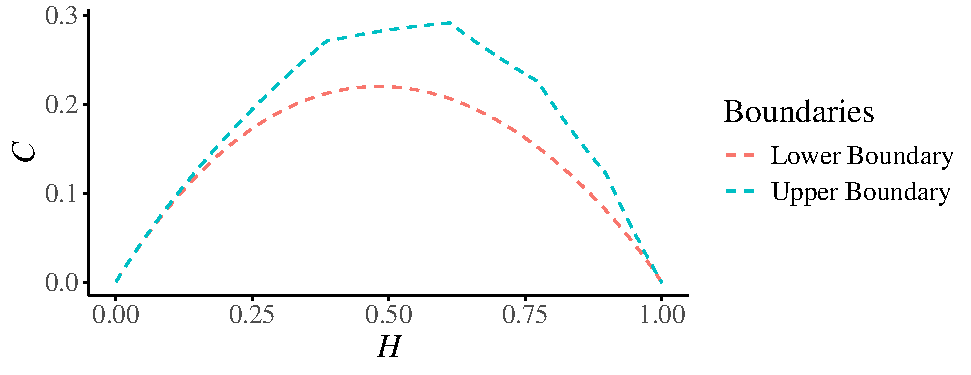
\includegraphics[width=0.7\textwidth]{complexity plane}
	\caption{Entropy Complexity Plane for Embedding dimension 3, 4,5, and 6}
	\label{fig:complexity}
\end{figure}


\begin{figure}[H]
	\centering
	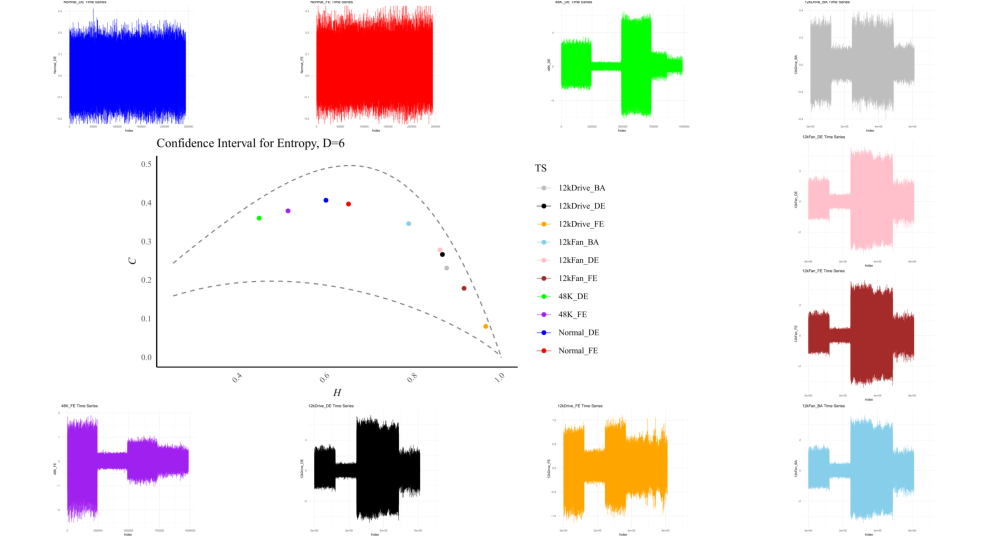
\includegraphics[width=0.7\textwidth]{combined plot}
	\caption{Time series plots and their points in the $H \times C$ plane for Embedding dimension 6}
	\label{fig:tentimeseries}
\end{figure}

\section{Asymptotic Distribution of the permutation entropy}\label{Sec:AsymptoticDistribution}
Ordinal patterns are a robust symbolic transformation method that enables the unveiling of latent dynamics in time series data. This approach involves constructing histograms of patterns and calculating both entropy and statistical complexity. According to the literature, determining the exact distribution of features derived from ordinal patterns is challenging; therefore, researchers have extensively investigated this distribution and its related statistical properties. Two types of statistical distributions are discussed in the literature: the empirical distribution and the asymptotic distribution.

The empirical distribution is used in conjunction with knowledge of the expected variability of entropy and complexity, allowing hypothesis tests to be performed for a wide variety of models according to the underlying dynamics. Results in this direction can be found in the literature~\cite{Chagas2022a, DeMicco2008, Larrondo2005, Larrondo2006}. In this approach, researchers construct empirical distributions directly from observed data, which reflect the actual frequencies of patterns or outcomes.

Furthermore, two types of asymptotic distributions are discussed: the first assumes that patterns are independent and identically distributed (multinomial model), while the second accounts for dependent patterns.

\subsection {Asymptotic Distribution of the Shannon Entropy under the Multinomial Model}\label{Subsec:Multinomial} 

%The Multinomial distribution describes how observations fall into categories when an adequate model is available. It is similar to the Multivariate normal distribution, which is one of the continuous Multivariate distributions. Furthermore, it has received considerable attention from researchers, both in theoretical studies and in applications related to discrete Multivariate distributions. 
%The normalized Shannon entropy, often employed in applications like permutation entropy, can be rigorously connected to its asymptotic distribution through the lens of statistical estimation theory. When estimating entropy from finite data, the plug-in estimator (computed directly from observed frequencies) converges to a normal distribution as the sample size $N\longrightarrow \infty$ even for dependent processes such as Markov chains. 
%%This asymptotic normality, demonstrated by Martin et al~\cite{M} 
%%% ACF Check the correct author/reference above
%%and Chagas et al~\cite{Chagas2022}, ensures that the estimator’s fluctuations around the true entropy value are Gaussian-distributed, with variance and bias determined by the underlying system’s dynamics. 
%The Statistical properties of entropy measures under Multinomial distributions are crucial for analyzing complex systems where entropy serves as a key descriptors. Rey at al~\cite{Rey2023} investigate the asymptotic distributions of various entropy measures specifically, the Rényi and Tsallis entropies of order $q$, as well as Fisher information when these are computed using maximum likelihood estimators of probabilities from Multinomial random samples. The authors demonstrate that the Tsallis entropy and Fisher information asymptotically follow a normal distribution, whereas the Rényi entropy does not exhibit asymptotic normality. Through simulation studies, the paper validates that these asymptotic models effectively describe a variety of data scenarios. Additionally, the study introduces test statistics for comparing different types of entropies derived from two samples, even when the samples have differing numbers of categories. An application of these tests to social survey data indicates that the results are consistent and offer a more general approach compared to traditional chi-squared tests. 


%In a subsequent study, Rey et al \cite{Rey2025} focus on the statistical complexity measure defined as the product of normalized Shannon entropy and the Normalized Jensen-Shannon divergence between a given probability distribution and the uniform distribution. 
%They derive the asymptotic distribution of this complexity measure under the assumption that the observed data follow a Multinomial distribution. Further the study demonstrates that, as the sample size increases, the distribution of the statistical complexity converges to a normal distribution, with its variance and bias determined by the dynamics of the underlying system. This result provides a theoretical foundation for using statistical complexity as a tool for analyzing systems where the probability distributions are estimated from finite samples. The results are validated with theoretical findings through numerical experiments, showing that the asymptotic normality holds even in scenarios where the Multinomial model is not strictly applicable, such as in applications involving Bandt and Pompe ordinal patterns. 

%Crucially, the convergence rate and limiting distribution depend on the system’s correlation structure, which deviates from the standard Multinomial case. However, they remain tractable through spectral analysis, which involves examining the eigenvalues and eigenvectors of the transition matrix or the distributions of ordinal patterns \cite{Chagas2022,PhysRevE.103.022215}. 
%%% ACF I don't recall that we mentioned "eigenvalues and eigenvectors of the transition matrix" in Chagas et al. (2022). Please be very careful when making such assertions.
%This connection underscores the reliability of normalized entropy measures in large data regimes while highlighting the need to account for dependence structures in finite sample applications.


%Imagine a sequence of $n$ independent trials, each resulting in precisely one outcome from a set of $k$ distinct possibilities labeled $\pi^1,\pi^2, \dots, \pi^k$ and so on. These outcomes are mutually exclusive, meaning only one can occur per trial, with respective probabilities $\mathbf{p}={\left\{p_1,p_2,\dots,p_k\right\}}$, such that $p_\ell \geq 0$ and $\sum^{k}_{\ell=1} {p_\ell =1}.$ The random vector $\mathbf{N}=(N_1,N_2,\dots, N_k)$ counts the number of occurrences of the events $\pi^1,\pi^2, \dots, \pi^k$ in the $n$ trials, with $N_\ell \geq0$ and $\sum^{k}_{\ell=1} {N_\ell =n}.$ A $\mathbf{n}$ is a sample from $\mathbf{N}$ and it has a $k-$variate vector of integer values $\mathbf{n}=(n_1,n_2,\dots,n_k).$ Then the joint distribution of $\mathbf{N}$ is 
%\begin{equation}
%	Pr(\mathbf{N=n})=Pr(N_1=n_1,N_2=n_2, \dots,N_k=n_k)=n!\prod_{\ell=1}^{k}\frac{{p_\ell}^{n_\ell}}{n_\ell !},
%\end{equation}   

%where $n_{\ell}\geq 0$ and $\sum_{\ell=1}^{k}n_{\ell}=n.$ This situation is denoted as $\mathbf{N}\sim \text{Mult}(n,\mathbf{p}),$ with $\mathbf{p}=(p_1,p_2,\dots,p_k)$ \cite{Chagas2022, Rey2023}.

%Under the conditions for applying the Bandt and Pompe technique, it is required that the sample size $n$ be sufficiently large, with $n\gg k$.

%Consider the random vector $\mathbf{N}\sim \text{Mult}(n,\mathbf{p}),$. Its first and second-order statistics (mean, variance, covariance, and correlation) are
%\begin{equation}
%	E(N_{\ell})=np_{\ell},
%\end{equation} 

%\begin{equation}
%	Var(N_{\ell})=np_{\ell}(1-p_{\ell}),
%\end{equation}

%\begin{equation}
%	Cov(N_{\ell},N_j)=-np_{\ell}p_j,
%\end{equation}

%\begin{equation}
%	\rho(N_{\ell},N_j)=\sqrt{\dfrac {p_{\ell}p_j}{(1-p_{\ell})(1-p_j)}},
%\end{equation}
%for every $1\leq \ell, j\leq k.   $
%In practical applications, the true probability distribution $\mathbf{p}$ governing a Multinomial system is typically unknown. 
%%% ACF As previously pointed many times, do not change the notation. You used \ell (correct), and then l (incorrect)
%Instead, estimators $\widehat{p}_\ell,$ are derived empirically by calculating the observed frequency of each event $\pi^l$ within the set of $k$ possible outcomes $\mathbf{\pi}=\pi^1,\pi^2, \dots, \pi^k$  across $n$ independent trials. These frequencies approximate the underlying probabilities, enabling inference about the system’s behavior. This maximum likelihood estimator (MLE) aligns with the empirical estimator derived from first-moment matching of the distribution. Due to its consistency, asymptotic normality, and computational tractability under regularity conditions, it remains the predominant choice in applied statistical modeling.

%The maximum likelihood (ML) estimator of $p_{\ell}$ is the relative frequency  $\widehat{p_{\ell}}=N_{\ell}/n, 1\leq \ell \leq k,$ and the distribution of $n \widehat{\mathbf{p}}$ follows $\text{Mult}(n,\mathbf{p})$. From the general properties of ML estimators, if  $\mathbf{\widehat{p}}$ is the ML estimator of $\mathbf{p}$, then for any function $g(\mathbf{p})$, the ML estimator of $g(\mathbf{p})$, denoted $\widehat g({\mathbf{p}}),$ is given by $g(\widehat{\mathbf{p}}).$ This property can be applied to derive the asymptotic distribution of Shannon's entropy.   

%Shannon entropy quantifies the level of disorder within a system. When the system's behavior is entirely predictable, the Shannon entropy reaches its minimum, indicating complete knowledge of future observations. Conversely, when the system follows a uniform distribution where all possible outcomes have equal probability, the entropy is maximized, reflecting minimal knowledge about the system's behavior. Chagas et al. \cite{Chagas2022} have analyzed the asymptotic distribution of Shannon entropy in their study.


%Rey et al.~\cite{Rey2023} investigated the asymptotic distribution of the estimators defined above, and provided the following formulation.

%Let  $\mathbf{Z}\sim N(\mathbf{\mu},\sum),$ be a $k-$dimensional multivariate normal distribution with mean vector $\mu \in \mathbb{R}^k$ and covariance matrix $\sum=(\sigma_{{\ell}{j}})$. Then, for any $\mathbf{a} \in \mathbb{R}^k,$ the linear combination $W=\mathbf{a}^T\mathbf{Z},$ is normally distributed as:
%\begin{equation}
%	W\sim N\Big(\mathbf{a}^T\bm{\mu},\sum_{\ell=1}^{k}a_\ell^2 \sigma_{{\ell}{\ell}}+2\sum_{j=1}^{k-1}\sum_{\ell=j+1}^{k} a_\ell a_j\sigma_{{\ell}{j}}\Big).
%\end{equation}
%The estimated Shannon entropy is defined as:
%\begin{equation}
%	H_s(\widehat{\mathbf{p}})=-\sum_{\ell=1}^{k}\widehat{p_\ell}\log\widehat{p_\ell}.
%\end{equation}
%The asymptotic variance $\widehat{\sigma}^2$ of the entropy estimator is given by:
%\begin{equation}
%	\widehat{\sigma}^2=\dfrac{1}{n}\sum_{\ell=1}^{k}p_\ell(1-p_\ell)(\log p_\ell+1)^2-\dfrac{2}{n}\sum_{j=1}^{k-1}\sum_{\ell=j+1}^{k}p_\ell p_j(\log p_\ell+1)(\log p_j+1).
%\end{equation}
%These formulas serve as the basis for the subsequent case study in our research.

The multinomial distribution models counts of observations in $k$ mutually exclusive categories $\pi^1,\pi^2,\dots,\pi^k$ from $n$ independent trials, with probability vector $\mathbf{p} = (p_1, p_2, \dots, p_k)$, $p_\ell \ge 0$, $\sum_{\ell=1}^k p_\ell = 1$. Let $\mathbf{N} = (N_1, \dots, N_k)$ denote category counts, $\sum_{\ell=1}^k N_\ell = n$. Its probability mass function is
\[
\Pr(\mathbf{N} = \mathbf{n}) = n! \prod_{\ell=1}^k \frac{p_\ell^{n_\ell}}{n_\ell!}, \quad \mathbf{N} \sim \mathrm{Mult}(n, \mathbf{p}),
\]
with moments
\[
E(N_\ell) = n p_\ell, \quad
\mathrm{Var}(N_\ell) = n p_\ell (1-p_\ell), \quad
\mathrm{Cov}(N_\ell, N_j) = -n p_\ell p_j.
\]

The maximum likelihood (ML) estimator $\widehat{p}_\ell = N_\ell / n$ satisfies $n\widehat{\mathbf{p}} \sim \mathrm{Mult}(n,\mathbf{p})$. For any smooth function $g(\mathbf{p})$, the plug-in estimator $\widehat{g}(\mathbf{p}) = g(\widehat{\mathbf{p}})$ is also ML, enabling the asymptotic distribution of Shannon entropy
\begin{equation}
	H(\mathbf{p}) = -\sum_{\ell=1}^k p_\ell \log p_\ell,
	\label{eq:AsymEntropy}
\end{equation}
to be derived from the asymptotic normality of $\widehat{\mathbf{p}}$ as $n \to \infty$.
The Shannon's entropy of a multinomial distributed random variable is bounded between 0 and $\ln k$. The minimum is attained when $p_{\ell}=1$ for some $1\leq \ell \leq k$ and $p_j=0$ for every $j\ne \ell$. The expression is maximized by $p_{\ell}=1/k$ for every $1\leq \ell \leq k$.  

Further, asymptotic distribution can be described as follows. Let $X_n=(X_{1n},X_{2n},\dots,X_{kn})$ be a sequence of independent and identical distributed random vectors, with distribution $\text{Mult}(n,\mathbf{p})$. If $\widehat{\mathbf{p}}$ denotes the vector of sample proportions, and 

\[\mathbf{Y}_n=\sqrt{n}(\widehat{\mathbf{p}}-\mathbf{p})\] 

then

\[E(\mathbf{Y}_n)=0,\]
\[\text{Cov}(\mathbf{Y}_n)=\mathbf{D_p}-\mathbf{pp}^T,\]
where $\mathbf{D_p}=\text{Diag}(p_1,p_2,\dots,p_k)$, and the superscript $T$ denotes transposition. The asymptotic distribution of $\mathbf{Y}_n$ is multivariate normal with mean vector $0$ and covariance matrix $\mathbf{D_p}-\mathbf{pp}^T$, denoted as
%%% ACF Check how I wrote it
%The notation for this can be shown as follows.
%
\begin{equation}
	\mathbf{Y}_n \xrightarrow{\mathscr{D}} N(\mathbf{0}, \mathbf{D_p}-\mathbf{pp}^T).
	\label{eq:Cov} 
\end{equation}
 
Our focus is on the statistical properties of $H(\mathbf{p})$ when $\mathbf{p}$ is replaced by its maximum likelihood estimate $\widehat{\mathbf{p}} = (\widehat{p}_1, \widehat{p}_2, \dots, \widehat{p}_k)$. The problem thus reduces to determining the distribution of $H(\widehat{\mathbf{p}})$.

\begin{align}
	H(\widehat{\mathbf{p}})
	&= -\sum_{\ell=1}^k \widehat{p}_\ell \log \widehat{p}_\ell \nonumber \\
	&= -\sum_{\ell=1}^k \frac{N_\ell}{n} \log \frac{N_\ell}{n} \nonumber \\
	&= \log n - \frac{1}{n} \sum_{\ell=1}^k N_\ell \log N_\ell,
\end{align}
under $N=(N_1,N_2,\dots,N_k)\sim \text{Mult}(n,\mathbf{p})$

For the asymptotic distribution case, we refer to the Delta Method theorems and their multivariate version.

\theoremstyle{plain}
\newtheorem{theorem}{Theorem}

\begin{theorem}[Delta Method, univariate]
	Let $X_n$ be a sequence of independent and identically distributed random variables such that 
	$\sqrt{n}(X_n - \theta) \xrightarrow{\mathscr{D}} N(0,\sigma^2)$. 
	Consider a function $h$ such that $h'(\theta)$ exists and $h'(\theta)\neq 0$. 
	Then,
	\[
	\sqrt{n}\,[h(X_n)-h(\theta)] \xrightarrow{\mathscr{D}} N\!\left(0,\,\sigma^2 [h'(\theta)]^2\right).
	\]
\end{theorem}

\begin{theorem}[Delta Method, multivariate]
	Let $\mathbf{X}_n= (X_{1n}, X_{2n}, \dots, X_{kn})$ be a sequence of independent and identically distributed random vectors such that 
	\[
	\sqrt{n}\,(\mathbf{X}_n - \boldsymbol{\theta}) \xrightarrow{\mathscr{D}} N_k(\mathbf{0},\Sigma),
	\]
	where $\boldsymbol{\theta} = (\theta_1,\theta_2,\dots,\theta_k)$ and $\Sigma$ is the covariance matrix. 
	Suppose that $h:\mathbb{R}^k \to \mathbb{R}^m$ is continuously differentiable in a neighborhood of $\boldsymbol{\theta}$, with Jacobian matrix
	\[
	B = \left( \frac{\partial h_i}{\partial \theta_j} \right)_{i,j=1}^k,
	\]
	which is non-singular at $\boldsymbol{\theta}$. Then,
	\[
	\sqrt{n}\,\big(h(\mathbf{X}_n)-h(\boldsymbol{\theta})\big) \xrightarrow{\mathscr{D}} N_m\!\left(\mathbf{0},\, B \Sigma B^T\right).
	\]
\end{theorem}

Further, covariance matrix of Equation~\eqref{eq:Cov} can be expressed as 
%%% ACF Use \eqref when referring to equations
%%% ACF Do not leave blank lines between elements of the same sentence
\begin{equation}
	(\mathbf{D_p}-\mathbf{pp}^T)_{\ell j} =
	\begin{cases}
		p_{\ell}(1-p_{\ell}), & \text{if } \ell = j, \\[6pt]
		-\,p_{\ell}p_{j}, & \text{if } \ell \neq j,
	\end{cases}
\end{equation}
for $1\leq {\ell}, j\leq k.$
Even for dependent processes (e.g., Markov chains), normalized Shannon entropy converges to a normal distribution with variance determined by the covariance structure of $\widehat{\mathbf{p}}$. 
%Rey et al.~\cite{Rey2023} showed that Tsallis entropy and Fisher information are asymptotically normal, whereas Rényi entropy is not, and proposed two-sample entropy comparison tests for distributions with unequal category counts. 

Rey et. al.~\cite{Rey2025} derived the asymptotic distribution of statistical complexity, defined as normalized Shannon entropy times normalized Jensen–Shannon divergence from the uniform distribution under the multinomial model. They demonstrated convergence to normality, with variance and bias reflecting the system’s dynamics. Numerical studies confirm robustness even when the multinomial model is approximate, such as in Bandt–Pompe ordinal patterns. 

We refer the asymptotic equation for the mean and variance provided by Rey et. al.~\cite{Rey2025} for our research work.
%%% ACF The following is strange; the left part depends on p, the right-hand side depends on \widehat p
\begin{equation}
	\mu_{n,\mathbf{p}}	= H(\widehat{\mathbf{p}})
	= -\sum_{\ell=1}^k \widehat{p}_\ell \log \widehat{p}_\ell 
	\label{eq:AsympMean}
\end{equation}  

%%% ACF Is the verb missing?
The above equation~\eqref{eq:AsympMean} normally distributed with mean $H(\mathbf{p})$ and variance $\sigma^2_{n,\mathbf{p}},$ where
\begin{equation}
	\sigma^2_{n,\mathbf{p}}=\dfrac{1}{n}\sum_{\ell=1}^{k}p_\ell(1-p_\ell)(\log p_\ell+1)^2-\dfrac{2}{n}\sum_{j=1}^{k-1}\sum_{\ell=j+1}^{k}p_\ell p_j(\log p_\ell+1)(\log p_j+1).
\end{equation}
%When dependence exists, convergence rates and variances deviate from the independent case but remain tractable via spectral analysis \cite{Chagas2022,PhysRevE.103.022215}, providing a rigorous basis for entropy-based analysis of finite-sample categorical data.
For practical purposes, given $n$ sufficiently large, we can use that 
%%% ACF That equation describes a deterministic object that does not have a normal distribution
Equation~\ref{eq:AsymEntropy} has a normal distribution with mean equal to $H(\widehat{\mathbf{p}})$ and variance equal to $\sigma^2_{\mathbf{p}}/n.$ In addition, for $\alpha \in (0,1)$ and $n$ sufficiently large, the $(1-\alpha)$\SI {100}{\percent} confidence interval for estimated entropy is shown as below.

\begin{equation}
	H(\widehat{\mathbf{p}})\pm \dfrac{Z_{\alpha/2}\widehat{\sigma}_{\widehat{\mathbf{p}}}}{\sqrt{n}},
	\label{eq:ConfidenceInterval}
\end{equation}
where $Z_{\alpha/2}$ is the $\alpha/2$-quantile of a standard normal random variable.


\subsection{Asymptotic distribution of Permutation Entropy under the pattern dependence}\label{Subsec:PatternDependence}

As we discussed earlier, real-valued time series $\mathbf{x}=\{x_1,x_2,...,x_{n+D-1}\}$  transform into the series symbols $\mathbf{{\pi}}=({\pi}_1, {\pi}_2,\dots, {\pi}_n)$ from sub-sequences of embedding dimension $D$, where we considered $D!=k$. Due to the overlapping of time windows, the ordinal patterns which we calculate are dependent. 
%%% ACF Use \dots and correct punctuation
For $i=1,2,...k$, let $p_i$ be the probability of observing the state $\pi_i$, denote the vector probabilities, $\mathbf{p}={\left\{p_1,p_2,\dots,p_k\right\}}$ and express as $\mathbf{D_p}=\text{Diag}(p_1,p_2, \dots, p_k)$ the diagonal matrix. 
The transition probability of reaching state $\pi_j$ at time 
%%% ACF Is this the same \ell as before?
$t+\ell$ from the state $\pi_i$ at time $t$, for $\ell=1,2,\dots,D-1$, is denoted by $p^{(\ell)}_{ij}$. These transition probabilities can be collected in the matrix $\mathbf{Q}^{(\ell)}$ whose elements are  $p^{(\ell)}_{ij}$. As describe in the Rey et al.~\cite{Rey2023a} when $n$ is sufficiently large, asymptotic variance of the Shannon entropy defined as follows:
%\begin{equation}
	%\sigma^2_{\bm{p}}=\sum_{i=1}^{k}(\bm{\Sigma}_{\bm{p}})_{ii}+2\sum_{i=1}^{k-1}\sum%_{j=i+1}^{k}(\bm{\Sigma}_{\bm{p}})_{ij}=\sum_{i=1}^{k}(\ln p_i+1)^2
%\times \left[ p_i-(2D-1)p^2_i+2\sum_{\ell=1}^{D-1}\bm{Q}^{(\ell)}_{ii}\right] - %2\sum_{i=1}^{k-1}\sum_{j=i+1}^{k} (\ln p_i+1)(\ln p_j+1) \left[(2D-1)p_i %p_j-\sum_{\ell=1}^{D-1}\left(\bm{Q}^{(\ell)}_{ij}+\bm{Q}^{(\ell)}_{ji}\right)\right].
%\end{equation}
\begin{equation}
	\begin{split}
		\widehat{\nu}^2_{\widehat{\mathbf{p}}} = & \sum_{i=1}^{k}(\ln p_i + 1)^2 
		\left[ p_i - (2D - 1)p_i^2 + 2\sum_{\ell=1}^{D-1} \mathbf{Q}^{(\ell)}_{ii} \right] \\
		& - 2 \sum_{i=1}^{k-1} \sum_{j=i+1}^{k} (\ln p_i + 1)(\ln p_j + 1) \\
		& \quad \times \left[ (2D - 1)p_i p_j - \sum_{\ell=1}^{D-1} \left( \mathbf{Q}^{(\ell)}_{ij} + \mathbf{Q}^{(\ell)}_{ji} \right) \right].
	\end{split}
	\label{eq:asympvar}
\end{equation} 

%%% ACF The first sentence repeats the last of the previous paragraph
Asymptotic variance of the Shannon entropy of ordinal patterns considering their correlation structure is given in Equation~\ref{eq:asympvar}.
%%% ACF Again, a deterministic quantity does not have a normal distribution
For practical purpose, given $n$ is sufficiently large, we can use $H(\mathbf{p})$ has a normal distribution with mean equal to $H(\widehat{\mathbf{p}})$ and variance equal to $\nu^2_{\mathbf{p}}/n$. 

In addition to that, for $\alpha\in(0,1)$ and $n$ sufficiently large, the $(1-\alpha)\SI{100}{\percent}$ confidence interval of $H(\mathbf{p})$ is given by, 
\begin{equation}
  H(\widehat{\mathbf{p}})\pm \dfrac{Z_{\alpha/2}\nu_{\mathbf{p}}}{\sqrt{n}},
  \label{eq:ConfidenceInterval}
\end{equation} 
where $Z_{\alpha/2}$ is the $\alpha/2$-quantile of a standard normal random variable.

For convenience, Equation~\ref{eq:ConfidenceInterval} is referred to and defined as follows.
\begin{equation}
	H(\widehat{\mathbf{p}})\pm \textbf{Semi Length},
	\label{eq:CI}
\end{equation} 
where $\textbf{Semi Length}=\dfrac{Z_{\alpha/2}\nu_{\mathbf{p}}}{\sqrt{n}}$

\subsection{Asymptotic Variance of Statistical Complexity $C(\widehat{\mathbf{p}})$}\label{Subsec:AsympVarComplexity}

%%% ACF If it is estimated, it is a constant and its variance is zero
The variance of the estimated complexity, $C(\widehat{\mathbf{p}})$, has two estimators:
\begin{itemize}
	%%% ACF Provide the expression taking care to make the notation match previous definitions
	\item \textbf{Multinomial model variance}, denoted as $\widehat{\omega}^2_{\widehat{\mathbf{p}}}$, which assumes independent ordinal patterns.
	\item \textbf{Serial dependence variance}, denoted as $\widehat{\eta}^2_{\widehat{\mathbf{p}}}$.
\end{itemize}
To estimate the serial dependence variance, we first compute the ratio
$$
a = \dfrac{\widehat{\nu}^2_{\widehat{\mathbf{p}}}}{\widehat{\sigma}^2_{\widehat{\mathbf{p}}}},
$$
%%% ACF Provide the equations
where $\widehat{\nu}^2_{\widehat{\mathbf{p}}}$ is the variance of entropy under serial dependence, and $\widehat{\sigma}^2_{\widehat{\mathbf{p}}}$ is the variance of entropy under independence.
Then, the serial dependence statistical complexity variance is calculated by scaling the Multinomial statistical complexity variance:
\[
\widehat{\eta}^2_{\widehat{\mathbf{p}}} = a \times \widehat{\omega}^2_{\widehat{\mathbf{p}}}.
\]
This approach allows to calculate the estimated statistical complexity variance for serial dependence.


\subsection{Other types of Entropy}
Moreover, other types of descriptors, such as Rényi entropy~\cite{renyi1961measures}, Tsallis entropy~\cite{tsallis1988possible}, and Fisher information~\cite{frieden2004science}, have been proposed to extract additional information that is not captured by Shannon entropy.
From these entropy measures, Fisher information has garnered more attention due to its unique properties. Fisher information is defined as the average logarithmic derivative of a continuous probability density function.

For discrete probability distributions, Fisher information can be approximated by calculating the differences between probabilities of consecutive distribution elements. A key distinction between Shannon entropy and Fisher information lies in their focus: Shannon entropy quantifies the overall unpredictability of a system, while Fisher information measures the rate of change between consecutive observations, making it more sensitive to small changes and perturbations.

The following equations define Tsallis entropy $	(H_{T}^{q}(\widehat{\mathbf{p}}))$, Rényi entropy $(H_{R}^{q}(\widehat{\mathbf{p}}))$, and Fisher information measures $(H_{F}(\widehat{\mathbf{p}}))$ \cite{sanchez2009discrete} :
\begin{equation}
	H_{T}^{q}(\widehat{\mathbf{p}})=\sum_{\ell=1}^{k}\dfrac{\widehat{p_\ell}-\widehat{p_\ell}^q}{q-1},
\end{equation}
where the index $q\in \mathbb{R}\backslash \{1\}$
\begin{equation}
	H_{R}^{q}(\widehat{\mathbf{p}})=\dfrac{1}{1-q} \log \sum_{\ell=1}^{k}{\widehat{p_\ell}}^q,
\end{equation}
where the index $q\in \mathbb{R}^{+}\backslash \{1\}$
\begin{equation}
	H_F(\widehat{\mathbf{p}})=F_0\sum_{\ell=1}^{k-1}\Big(\sqrt{\widehat{p_\ell}_{+1}}-\sqrt{\widehat{p_\ell}}\Big)^2 ,
\end{equation}
where the re-normalization coefficient is $F_0=4$ \cite{sanchez2009discrete}

\section{Case Study of Asymptotic Distribution of the Shannon Entropy under pattern dependence and independence} \label{Sec:CaseStudy} 

Statistical complexity is defined as the product of two normalized quantities:
\begin{itemize}
	\item The Shannon entropy,
	\item The Jensen-Shannon distance between the observed probability distribution and the uniform distribution. 
\end{itemize}

In this section we discuss two key aspects with real world scenario:
\begin{enumerate}
	\item \textbf{Significance of Asymptotic Distributions}: Why understanding large-sample behavior matters for statistical inference,
%	\item \textbf{Multinomial Model Framework}: Derivation of the asymptotic distribution for statistical complexity under Multinomial assumptions
	\item \textbf{Practical Formula}: A working equation for calculating the asymptotic distribution of complexity.
\end{enumerate}

As a case study for our work, we consider data from the Bearing Data Center and the seeded fault test data from Case Western Reserve University, School of Engineering. The datasets includes ball bearing test data for normal bearings as well as single-point defects on the fan end and drive end. Data were collected at a rate of $48,000 (48k$ drive-end) data points per second during bearing tests. Each file contains motor loads $(0, 1, 2,$ and $3)$, drive-end vibration data, and fan-end vibration data. The approximate motor speeds in RPM during testing: $1797, 1772, 1750,$ and $1730$. For our case study, we consider two time series (Normal Baseline and $48k$ Drive-End) with a motor load of $0$ and an RPM of $1797$. 

The primary objective of this study is to detect malfunctioning machinery by analyzing two time series using ordinal patterns. We introduce a distance metric based on the ordinal structure of the segments to quantify similarity. This metric facilitates the identification of faulty machines across various embedding dimensions, ranging from $3$ to $6$. For this case study, we employ an embedding dimension of $3$ for convenience; subsequent analyses will extend to the remaining dimensions to compare results. Permutation entropy under asymptotic conditions is computed by considering the probability distribution of ordinal patterns. The results are further analyzed using the complexity–entropy plane, providing insights into the system's dynamics.

Initially, we analyzed complete datasets from two time series: one comprising 250,000 data points representing the normal baseline at motor load 0, and another containing 2,540,000 data points from the 48k drive end under the same motor load. We computed the entropy and complexity measures for these entire datasets, followed by the calculation of the asymptotic variance as defined in Section~\ref{Subsec:PatternDependence}. This asymptotic variance was then used to determine the confidence interval for entropy (Equation is defined in~\ref{eq:ConfidenceInterval}). The calculation of the semi-length of the interval is given by Equation~\ref{eq:CI}. The final results are presented in Table~\ref{tab:EnComplexResults}.


\begin{table}[H]
	\centering
	\begin{tabular}{llcr}
		\toprule
		Entropy  & Complexity  & $\sigma_{\bm{p}}$ & Semi Length \\
		\midrule
		$0.665235$ & $0.226447$ & $0.358893$ & $0.000441$\\ 
		$0.772973$ & $0.170954$ & $0.324376$ & $0.001287$\\
		\bottomrule
	\end{tabular}
	\caption{Entropy Complexity Results}
	\label{tab:EnComplexResults}
\end{table}

Subsequently, we segmented the data into batches of $10,000$ points, categorizing them as either `Normal` or `48k Drive End`. We then performed a batch wise comparison of entropy and complexity metrics to identify fault data segments. 
The normal dataset comprises $25$ batches, all corresponding to motor load $0$, while the $48k$ drive end dataset includes $254$ batches. Due to the extensive volume of entropy and complexity data generated, the complete results table is not included in this report. However, the entropy–complexity plane effectively illustrates both batch-wise and full-data analyses. As depicted in Figure \ref{fig:EntopyComplexity Plane} below, faulty machines form a distinct cluster in the entropy–complexity plane, highlighting their deviation from normal operational patterns. 
It is clear from the graph that there are both overlapping and non-overlapping confidence intervals. This indicates that some machines differ significantly, while others do not. The main purpose of our experiment is to identify faulty machines. Therefore, we highly recommend extending these results by increasing the embedding dimension to better understand the final outcomes. The general framework of this experiment is also provided in this chapter to clarify the main objective of the research.

\begin{figure}[hbt]
	\centering
	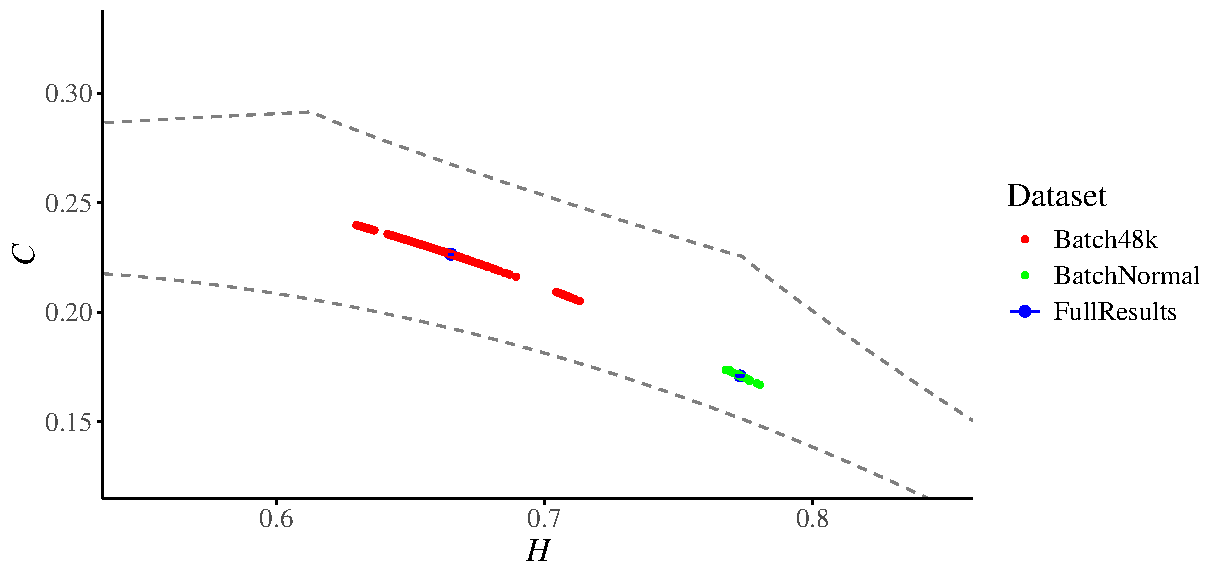
\includegraphics[width=0.8 \textwidth]{confidence_interval}
	\caption{Entropy Complexity Plane}
	\label{fig:EntopyComplexity Plane}
\end{figure}

In addition to this we analyze the full data results for higher embedding dimension $D=6$.
	\begin{figure}[hbt]
	\centering
	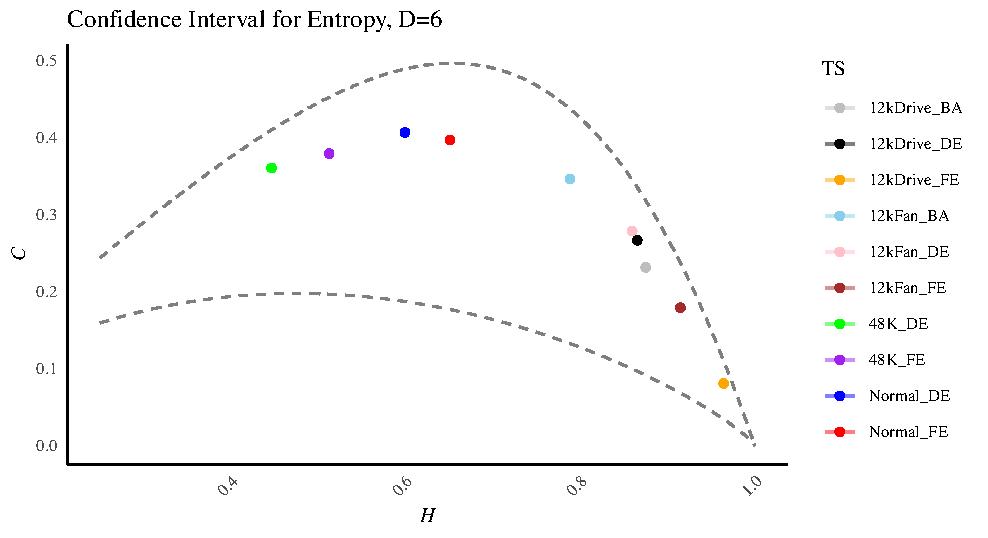
\includegraphics[width=0.8 \textwidth]{Confidence Interval}
	\caption{Entropy Complexity Plane for $D=6$}
	\label{fig:EntopyComplexity Plane D=6}
\end{figure}

Because the original case study involved a large sample size, we computed entropy and statistical complexity for smaller sample sizes of 100, 1000, and 2000. These values were then analyzed using both the Multinomial and Serial Dependence models. The analysis clearly demonstrates the confidence intervals for both entropy and complexity.	

\begin{figure}[H]
	\centering
	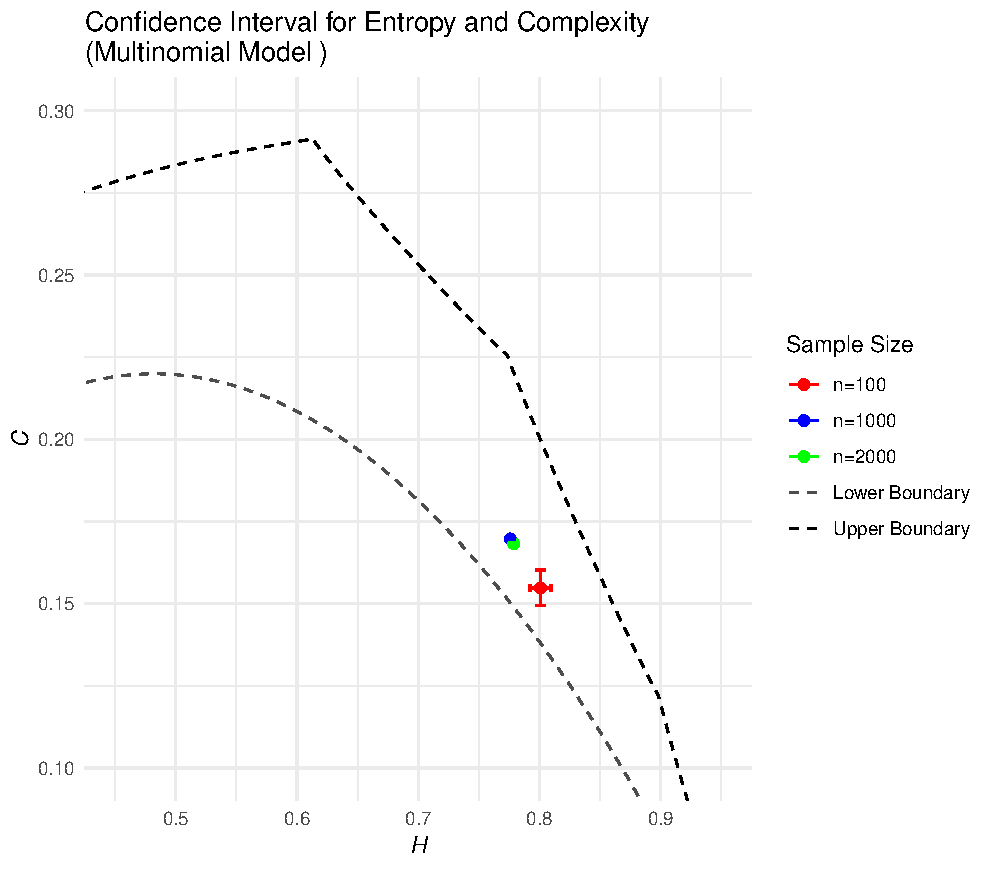
\includegraphics[width=0.8 \textwidth]{CI for Multinomial model}
	\caption{Confidence Interval for Multinomial Model}
	\label{fig:CIMultinorm}
\end{figure}

\begin{figure}[H]
	\centering
	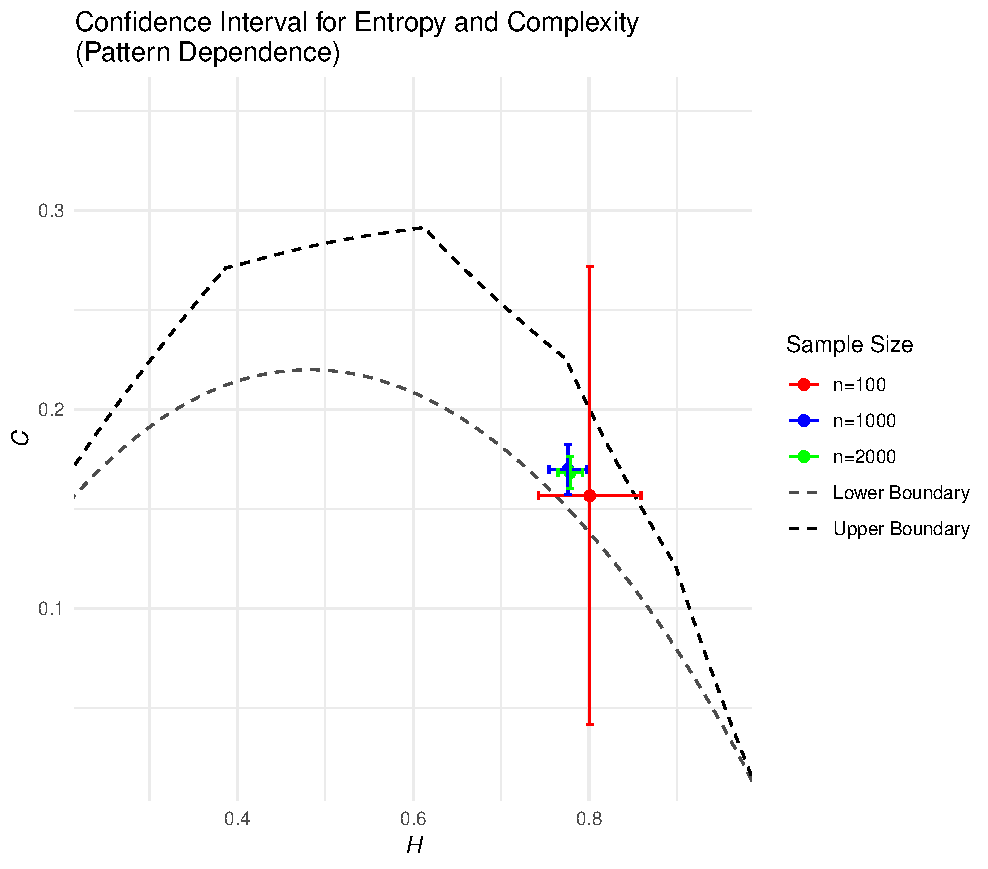
\includegraphics[width=0.7 \textwidth]{CI for pattern dependence}
	\caption{Confidence Interval Pattern Dependence model}
	\label{fig:CIDependence}
\end{figure}

The general framework for analyzing entropy-complexity planes with confidence intervals are given as follows.
\begin{enumerate}
	\item \textbf{Calculate Entropy (H) and Complexity (C):} 
	appropriate estimator are Shannon entropy, statistical complexity measures 
	\item \textbf{Compute Confidence Intervals:}
	Generate multiple resampled datasets to estimate the variance of $H$ and $C$.
	\item \textbf{Plot on Entropy-Complexity Plane:}
	\begin{itemize}
		\item Axes:x-axis: Entropy $(H)$, y-axis: Statistical complexity $(C)$
		\item Data Points: Plot individual or aggregated results.
		\item Confidence Regions: Represent uncertainty 
	\end{itemize}
	
	\item \textbf{Interpretation}
	\begin{table}[H]
		\centering
		\begin{tabular}{cr}
			\toprule
			Region of Plane  & Interpretation  \\
			\midrule
			High $H$ and High $C$ & Complex, structured systems \\ 
			Low $H$ and Low $C$ & Simple, predictable systems \\
			High $H$ and Low $C$ & Random/noisy systems \\
			Low $H$ and High $C$ & Non-random systems \\ 
			\bottomrule
		\end{tabular}
	\end{table}
	
	\item \textbf{Statistical testing:}
	\begin{itemize}
		\item Compare confidence intervals between groups to assess significant differences.
		\item Overlapping intervals $\rightarrow$ {No significant difference}.
		\item Non-overlapping intervals $\rightarrow$ Potential significance.
	\end{itemize}
\end{enumerate}







